% Created by tikzDevice version 0.12.5 on 2023-11-24 22:28:42
% !TEX encoding = UTF-8 Unicode
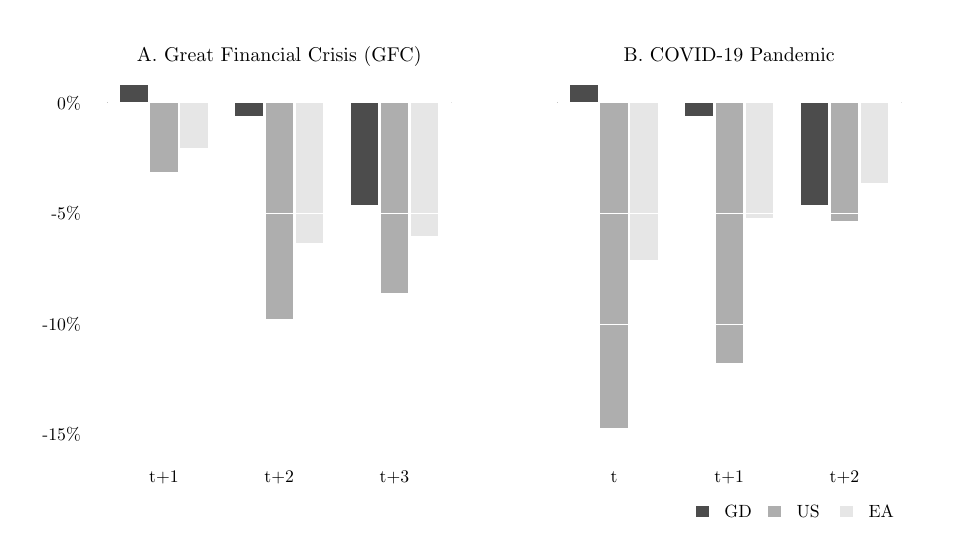
\begin{tikzpicture}[x=1pt,y=1pt]
\definecolor{fillColor}{RGB}{255,255,255}
\path[use as bounding box,fill=fillColor,fill opacity=0.00] (0,0) rectangle (325.21,180.67);
\begin{scope}
\path[clip] (  0.00,  0.00) rectangle (162.61,180.67);
\definecolor{fillColor}{gray}{0.30}

\path[fill=fillColor] ( 33.40,153.48) rectangle ( 43.31,159.88);
\definecolor{fillColor}{RGB}{174,174,174}

\path[fill=fillColor] ( 44.31,153.48) rectangle ( 54.22,128.67);
\definecolor{fillColor}{RGB}{230,230,230}

\path[fill=fillColor] ( 55.21,153.48) rectangle ( 65.13,137.14);
\definecolor{fillColor}{gray}{0.30}

\path[fill=fillColor] ( 75.04,153.48) rectangle ( 84.96,148.71);
\definecolor{fillColor}{RGB}{174,174,174}

\path[fill=fillColor] ( 85.95,153.48) rectangle ( 95.86, 75.50);
\definecolor{fillColor}{RGB}{230,230,230}

\path[fill=fillColor] ( 96.85,153.48) rectangle (106.77,102.79);
\definecolor{fillColor}{gray}{0.30}

\path[fill=fillColor] (116.68,153.48) rectangle (126.60,116.76);
\definecolor{fillColor}{RGB}{174,174,174}

\path[fill=fillColor] (127.59,153.48) rectangle (137.50, 84.74);
\definecolor{fillColor}{RGB}{230,230,230}

\path[fill=fillColor] (138.49,153.48) rectangle (148.41,105.51);
\end{scope}
\begin{scope}
\path[clip] (  0.00,  0.00) rectangle (325.21,180.67);
\definecolor{drawColor}{RGB}{0,0,0}

\node[text=drawColor,anchor=base,inner sep=0pt, outer sep=0pt, scale=  0.64] at ( 49.26, 16.32) {t+1};

\node[text=drawColor,anchor=base,inner sep=0pt, outer sep=0pt, scale=  0.64] at ( 90.90, 16.32) {t+2};

\node[text=drawColor,anchor=base,inner sep=0pt, outer sep=0pt, scale=  0.64] at (132.54, 16.32) {t+3};
\end{scope}
\begin{scope}
\path[clip] ( 28.80, 33.60) rectangle (153.01,161.47);
\definecolor{drawColor}{RGB}{0,0,0}

\path[draw=drawColor,line width= 0.4pt,line join=round,line cap=round] ( 28.80,153.48) -- (153.01,153.48);
\end{scope}
\begin{scope}
\path[clip] (  0.00,  0.00) rectangle (325.21,180.67);
\definecolor{drawColor}{RGB}{0,0,0}

\node[text=drawColor,anchor=base east,inner sep=0pt, outer sep=0pt, scale=  0.64] at ( 19.20, 31.40) {-15\%};

\node[text=drawColor,anchor=base east,inner sep=0pt, outer sep=0pt, scale=  0.64] at ( 19.20, 71.36) {-10\%};

\node[text=drawColor,anchor=base east,inner sep=0pt, outer sep=0pt, scale=  0.64] at ( 19.20,111.32) {-5\%};

\node[text=drawColor,anchor=base east,inner sep=0pt, outer sep=0pt, scale=  0.64] at ( 19.20,151.28) {0\%};
\end{scope}
\begin{scope}
\path[clip] ( 28.80, 33.60) rectangle (153.01,161.47);
\definecolor{drawColor}{RGB}{255,255,255}

\path[draw=drawColor,line width= 0.4pt,line join=round,line cap=round] ( 28.80, 33.60) -- (153.01, 33.60);

\path[draw=drawColor,line width= 0.4pt,line join=round,line cap=round] ( 28.80, 73.56) -- (153.01, 73.56);

\path[draw=drawColor,line width= 0.4pt,line join=round,line cap=round] ( 28.80,113.52) -- (153.01,113.52);

\path[draw=drawColor,line width= 0.4pt,line join=round,line cap=round] ( 28.80,153.48) -- (153.01,153.48);
\end{scope}
\begin{scope}
\path[clip] (  0.00,  0.00) rectangle (162.61,180.67);
\definecolor{drawColor}{RGB}{0,0,0}

\node[text=drawColor,anchor=base,inner sep=0pt, outer sep=0pt, scale=  0.72] at ( 90.90,168.60) {A. Great Financial Crisis (GFC)};
\end{scope}
\begin{scope}
\path[clip] (162.61,  0.00) rectangle (325.21,180.67);
\definecolor{fillColor}{gray}{0.30}

\path[fill=fillColor] (196.01,153.48) rectangle (205.92,159.88);
\definecolor{fillColor}{RGB}{174,174,174}

\path[fill=fillColor] (206.91,153.48) rectangle (216.83, 36.07);
\definecolor{fillColor}{RGB}{230,230,230}

\path[fill=fillColor] (217.82,153.48) rectangle (227.73, 96.74);
\definecolor{fillColor}{gray}{0.30}

\path[fill=fillColor] (237.65,153.48) rectangle (247.56,148.71);
\definecolor{fillColor}{RGB}{174,174,174}

\path[fill=fillColor] (248.55,153.48) rectangle (258.47, 59.47);
\definecolor{fillColor}{RGB}{230,230,230}

\path[fill=fillColor] (259.46,153.48) rectangle (269.37,111.92);
\definecolor{fillColor}{gray}{0.30}

\path[fill=fillColor] (279.29,153.48) rectangle (289.20,116.76);
\definecolor{fillColor}{RGB}{174,174,174}

\path[fill=fillColor] (290.19,153.48) rectangle (300.11,110.78);
\definecolor{fillColor}{RGB}{230,230,230}

\path[fill=fillColor] (301.10,153.48) rectangle (311.01,124.71);
\end{scope}
\begin{scope}
\path[clip] (  0.00,  0.00) rectangle (325.21,180.67);
\definecolor{drawColor}{RGB}{0,0,0}

\node[text=drawColor,anchor=base,inner sep=0pt, outer sep=0pt, scale=  0.64] at (211.87, 16.32) {t};

\node[text=drawColor,anchor=base,inner sep=0pt, outer sep=0pt, scale=  0.64] at (253.51, 16.32) {t+1};

\node[text=drawColor,anchor=base,inner sep=0pt, outer sep=0pt, scale=  0.64] at (295.15, 16.32) {t+2};
\end{scope}
\begin{scope}
\path[clip] (191.41, 33.60) rectangle (315.62,161.47);
\definecolor{drawColor}{RGB}{0,0,0}

\path[draw=drawColor,line width= 0.4pt,line join=round,line cap=round] (191.41,153.48) -- (315.62,153.48);
\definecolor{drawColor}{RGB}{255,255,255}

\path[draw=drawColor,line width= 0.4pt,line join=round,line cap=round] (191.41, 33.60) -- (315.62, 33.60);

\path[draw=drawColor,line width= 0.4pt,line join=round,line cap=round] (191.41, 73.56) -- (315.62, 73.56);

\path[draw=drawColor,line width= 0.4pt,line join=round,line cap=round] (191.41,113.52) -- (315.62,113.52);

\path[draw=drawColor,line width= 0.4pt,line join=round,line cap=round] (191.41,153.48) -- (315.62,153.48);
\end{scope}
\begin{scope}
\path[clip] (162.61,  0.00) rectangle (325.21,180.67);
\definecolor{fillColor}{gray}{0.30}

\path[fill=fillColor] (241.43,  7.86) rectangle (246.03,  4.02);
\definecolor{fillColor}{RGB}{174,174,174}

\path[fill=fillColor] (267.46,  7.86) rectangle (272.07,  4.02);
\definecolor{fillColor}{RGB}{230,230,230}

\path[fill=fillColor] (293.50,  7.86) rectangle (298.11,  4.02);
\definecolor{drawColor}{RGB}{0,0,0}

\node[text=drawColor,anchor=base west,inner sep=0pt, outer sep=0pt, scale=  0.64] at (251.79,  3.74) {GD};

\node[text=drawColor,anchor=base west,inner sep=0pt, outer sep=0pt, scale=  0.64] at (277.83,  3.74) {US};

\node[text=drawColor,anchor=base west,inner sep=0pt, outer sep=0pt, scale=  0.64] at (303.87,  3.74) {EA};

\node[text=drawColor,anchor=base,inner sep=0pt, outer sep=0pt, scale=  0.72] at (253.51,168.60) {B. COVID-19 Pandemic};
\end{scope}
\end{tikzpicture}
